\documentclass{article}
\usepackage[utf8]{inputenc}

%% Useful packages
\usepackage{helvet}
\renewcommand{\familydefault}{\sfdefault}
\usepackage{hyperref}
\usepackage{amsmath}
\usepackage{siunitx}
\usepackage[margin=1 in]{geometry}
\usepackage{indentfirst}
\usepackage{graphicx}
\usepackage{listings}
\setlength{\parskip}{0.5 em}
\usepackage{tikz}
\usetikzlibrary{shapes.geometric, arrows, decorations.pathreplacing}

%%%%%%%%% This is for editing only. %%%%%%%%%%%%%
\usepackage[todonotes={textwidth=1.5in},commentmarkup=footnote]{changes} % I use footnotes for comments be cause the default margin comments are often trucated if they occur too close to the bottom of the page.
\setaddedmarkup{\textcolor{teal}{#1}}
\setdeletedmarkup{\textcolor{red}{#1}}
%%%%%%%%%%%%%%%%%%%%%%%%%%%%%%%%%%%%%%%%%%%%%%%%%

\newenvironment{descriptions}
  {\par\vspace{\abovedisplayskip}\begin{tabular}{>{$}r<{$} @{$:{}$} l}}
  {\end{tabular}\par\vspace{\belowdisplayskip}}

\newenvironment{newdescriptions}
  {\begin{tabular}{>{$}r<{$} @{$:{}$} l}}
  {\end{tabular}}

\newcommand{\code}[1]{\texttt{#1}}

\newcommand{\cs}{\mathit{cs}} % This make TeX treat "cs" as a unit as opposed to typesetting it as the product of two variables "c" and "s".
\newcommand{\cd}{\mathit{cd}} % Similarly.

\title{\replaced{An Introduction to BioCro for Those Who Want to Add Models}{An introduction to BioCro for those who want to add models.}}
\author{Justin McGrath}

\begin{document}
\maketitle
\section{Plant growth as a system of differential equations}
\subsection{Overview}
BioCro is used to calculate aspects of plant growth, such as the \replaced{change in the mass of a}{current mass of the} plant, given \highlight[comment=or \emph{attributes}]{aspects} \replaced{of a}{about the} plant and its environment that are already known\deleted{, such as air temperature}.\comment{Dropping ``such as air temperature'' makes this seem less wordy; the immediately-following example clarifies the meaning.} For example, one can calculate leaf and stem mass over thermal time given measures of the climate (Figure \ref{fig:example}).
% * <jesse.mcgrath@gmail.com> 2017-07-19T17:37:22.667Z:
% 
% > Leaf and Stem
% lowercase, leaf and stem?
% 
% ^ <mcgrath.justin@gmail.com> 2017-07-21T14:11:10.210Z.

\begin{figure}[!h]
\centering
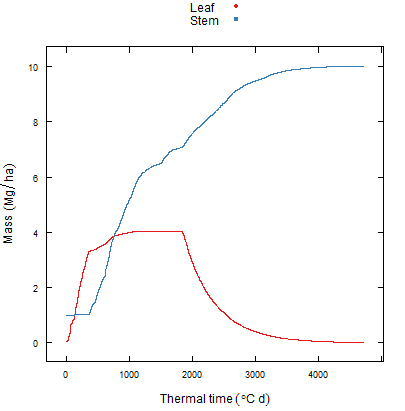
\includegraphics[width=0.3\textwidth]{example_gro.png}
\caption{\label{fig:example}Mass over time of willow.}
\end{figure}

\deleted{The use of the }BioCro is designed to reflect differential equation models. If you're already familiar with such models, skip to section \ref{sec:math_summary}.
% * <jesse.mcgrath@gmail.com> 2017-07-19T17:37:53.099Z:
% 
% > the
% delete "the".  Also the sentence is unusual.  The subject is "use" and verb is "is designed".  "BioCro is designed to reflect differential equation models" is probably better.
% 
% ^.

We'll call the set of all of the variables in the model (mass, temperature, wind speed, etc.) the \replaced{\emph{state}}{state}. We want to calculate \added{changes to [or \emph{in}]} the state \replaced{over}{for} some time period\comment{Or perhaps, more explicitly, ``\dots calculate the sequence of states over some time period \dots''}\replaced{---}{: }for example, every hour from June 1 to August 1.  We'll denote the state over the whole period\comment{Or ``\dots the collection [or \emph{sequence}] of states over the whole period \dots''?} as \replaced{$\mathbf{X}$}{$X$,}\comment{Using bold-faced X here is just a suggestion.  Bold-faced variables are often used in mathematical notations to indicate multidimensional quantities or vectors, and I think following this convention makes the notation clearer.  I haven't yet made this change throughout.}\comment{We may think of $\mathbf{X}$ as (1) a function $\mathbf{X}(t,v)$ on pairs $(t,v)$ of times and variable names that maps $(t,v)$ to the value of variable $v$ at time $t$; (2) a function $\mathbf{X}(t)$ mapping time $t$ to the state $\mathbf{X}_t$ at time $t$; (3) a function $\mathbf{X}(v)$ mapping each variable name $v$ to a function $\mathbf{X}_v(t)$ (which we might also call simply $v(t)$) which for each time $t$ yields the value of $v$ at time $t$.  This doesn't necessarily need to be spelled out for the reader, but it is useful to keep all this in mind in formulating the descriptions and attendant notation in what follows.  This also has a bearing on how $\mathbf{X}$ is represented in code.  That we use type \code{std::unordered\_map$<$std::string, std::vector$<$double$>$$>$} to represent $\mathbf{X}$ rather than, say, \code{std::vector$<$std::unordered\_map$<$std::string,double$>$$>$} suggests we have something close to conception (3) in mind.} and the state at a specific time\deleted{,} $t$\deleted{,} as \replaced{$\mathbf{X}_t$}{$X_t$}.\comment{It is confusing, and becomes increasingly so later on, to use $t$ to represent both the independent variable time on which the state depends and a particular value of that variable for some instant of time.  To emphasize the distinction, you could say ``\dots the state at a specific time $t_i$ [or time $t = t_i$] as $\mathbf{X}_{t_i}$.''}
% * <jesse.mcgrath@gmail.com> 2017-07-19T17:39:55.506Z:
%
% > We'll call the set of all of the variables in the model (mass, temperature, wind speed, etc) the state. We want to calculate the state for some time period: for example, every hour from June 1 to August 1.  We'll denote the state over the whole period as $X$, and the state at a specific time, $t$, as $X_t$.
%
% ^.

Some parts of the state are known \replaced{\emph{a priori}}{\textit{a priori}}\comment{Visually these are the same, but using the semantically-oriented command ``emph'' in preference to the visually-oriented ``textit'' command is the \TeX\ way of doing things.  After all, in typed text, underlining rather than italicizing is used to convey the same meaning.  Granted, this somewhat subtle distinction may be something of a fetish among \TeX\ gurus, and there are plenty of other places in \TeX\ where it seems common to resort to visually-based design, but I see no reason not to follow best-practice in this case.  And besides, it's two characters shorter!} for the entire period, and we'll denote \replaced{this component of the state}{these}\comment{or: ``\dots the [set of?] variables that comprise this component of the state \dots''} as $X_k$\comment{Corresponding to my earlier comment, we can think of $\mathbf{X}_k$ as (1) the restriction of $\mathbf{X}$ (as a function of $t$ and $v$) obtained by restricting the domain of $v$ to the set $k$ of variable names representing variables whose values are known for all time at the outset; (2) a function $\mathbf{X}_k(t)$ mapping time $t$ to the portion $\mathbf{X}_{t,k}$ of the state $\mathbf{X}_t$ that is known ahead of time; (3) the restriction of the function $\mathbf{X}(v)$ to variables $v\in k$ whose values for all time are known ahead of time.  (3) is most consistent with the conception of $\mathbf{X}$ as a plurality---namely, the collection of functions $\mathbf{X}_v(t)$ such that $v\in k$.} ($k$ for \replaced{\emph{known}}{known})\deleted{,} and denote the known state at time\deleted{,} $t$\deleted{,} as $X_{t,k}$. These values that are known beforehand are inputs of the model, and in \added{the} literature, people typically say that these variables \replaced{``}{"}drive" the model.

Some state variables can be calculated from other state variables without explicit dependence on time. For example, the total mass of the plant is the sum of leaf, stem\added{,}\comment{You use serial commas elsewhere, which is what most American style guides recommend, so I added one here.} and root masses.  This set of variables we'll denote as \replaced{$X_\cs$}{$X_{cs}$} (\replaced{$\cs$}{$cs$}  for \underline{c}alculated from \underline{s}teady state).\comment{Using ``steady state'' here seems a rather egregious appropriation of a term that usually means ``unvarying over time''.  I understand the desire for a convenient handle by which to refer to such variables, but this seems like an especially misleading one.  The best alternative I could come up with is ``statically dependent variable'', which, while perhaps not ideal, seems preferable}. 

Some variables must be calculated from \replaced{their}{the} rate of change, and therefore they depend explicitly on time.\comment{``Dependence on time'' is not what distiguishes these variables.  After all, the weather-related variables depend on time, and the model treats these as ``known'' variables.  Perhaps what you could say is ``Some variables may be calculated from the rate of change, and therefore they depend on time in a predictable way.''} For example, the rate of change of leaf mass is calculated from the photosynthetic rate, so the leaf mass at 10 \replaced{a.m.}{am}\comment{Alternatively, \textsc{a.m.} or \textsc{am}.} is the leaf mass at 9 \replaced{a.m.}{am} plus the rate of change\deleted{,}\comment{A comma here suggests the wrong order of operations.  Also, since you're introducing units of time, to be \emph{really} precise you should say ``\dots the rate of change in units of mass per second \dots \dots''.} times one hour (3600 seconds)\replaced{; that is,}{.}  \replaced{$\mathrm{mass}_\text{10\,am} = \mathrm{mass}_\text{9\,am} + \frac{d\mathrm{mass}}{dt} * \SI{3600}{s}$}{$mass_{10am} = mass_{9am} + \frac{dmass}{dt} * \SI{3600}{s}$}.\comment{Perhaps add, as a footnote, ``Here, $\frac{d\mathrm{mass}}{dt}$ is the \emph{average} rate of change of mass over the period from 9 a.m. to 10 a.m. in units of mass per second.  By the mean value theorem, this is equal to the derivative of leaf mass with respect to time at some instant (at least one) between 9 and 10 a.m.  In some forms of modeling, the derivative at the beginning of the time interval (at 9 a.m.) is taken as a resonable approximation of this value.''}\comment{I replaced $mass$, which \TeX\ typesets as if it were the product of the variables $m$, $a$, $s$, and $s$, with $\mathrm{mass}$, which \TeX\ typesets as a word.  The spacing problems with $mass$ are often not very noticable, especially with some lower-quality implementations of the $\LaTeX$ typesetter; but especially in the case of $dmass$, I think $d\textrm{mass}$ is clearer.} The variables we calculate from rates of change we'll denote as \replaced{$X_\cd$}{$X_{cd}$} (\replaced{$\cd$}{$cd$} for \underline{c}alculated from \underline{d}ifferential equations).


As with $X$ and $X_t$, to denote a specific time\added{,} a subscript $t$ is used: for example, \replaced{$X_{t, \cd}$}{$X_{t, cd}$}. Since each \replaced{$X_{t, \cd}$}{$X_{t,cd}$} depends on the previous value\comment{\emph{previous value:} This is the first time it is made abundantly clear that $t$ is intended to be a discrete variable, possibly even an integer-valued one, though the reference to ``every hour from June 1 to August 1'' in the third paragraph hints that it might be.  For clarity, it would be worthwhile adding a sentence before this one explaining this: ``For the purposes of our model, our time variable $t$ will be assumed to take on discrete values, starting with some intial time $t_0$ and continuing with times $t_1$, $t_2$, \dots, $t_i$, \dots, et cetera.''}, that is \replaced{$X_{t-1,\cd}$}{$X_{t-1, cd}$}, the initial value, \deleted{that is }\replaced{$X_{0, \cd}$}{$X_{0, cd}$}, must be given as input to the model.\comment{If we don't want to be locked into a time step size of 1 and an initial value of time 0, it would be better to notate this all as follows: ``Since each $X_{t_i, \cd}$ depends on the previous value, that is $X_{t_{i-1},\cd}$, the initial value, $X_{t_0, \cd}$, must be given as input to the model."}

We'll denote the \replaced{function that describes}{equations that describe} how to calculate steady-state variables ($X_{t,cs}$) from variables we know beforehand ($X_{t,k})$ as $g(X_{t,k})$.\comment{We can think of $\mathbf{g}$ as a collection of functions $g_v$ ($v\in \cs$) where each $g_v$ maps a collection of values for the known variables $k$ to a value for the variable $v$.  I assume this is close to how you are thinking when you say $g(X_{t,k})$ denotes ``the equations that describe \dots''.  If there are $m$ known variables and $n$ variables in $\cs$, then we can also think of $\mathbf{g}$ as a vector-valued vector function from the $m$-dimensional Euclidean space whose axes are labelled by the variables of $k$ to the $n$-dimensional Euclidean space whose axes are labelled by the variables of $\cs$.  I thought it was confusing to equate a state---$\mathbf{X}_{t,\cs}$---with $\mathbf{g}(\mathbf{X}_{t,k})$ immediately after you have referred to $\mathbf{g}(\mathbf{X}_{t,k})$ as a collection of equations.  This is perhaps not fundamentally different from using $\mathbf{g}(\mathbf{X}_{t,k})$ to denote both the function $\mathbf{g}$ itself and the value of that function for a particular value $\mathbf{X}_{t,k}$ of its argument, but the latter is such common practice that trying to use more precise notation begins to seem overly pendantic.  (See my following note on functional notation.)} Thus, \replaced{at any particular time $t_i$, $\mathbf{X}_{t_i,\cs} = g(\mathbf{X}_{t_i,k})$}{$X_{t,cs} = g(X_{t,k})$}.  \added{Note that $g$ does not depend on time $t$, only on the value of the ``known'' component $\mathbf{X}_k$ of the state $\mathbf{X}$ at some time $t_i$.  $g$ may be viewed as a collection of equations telling how to calculate the value of each variable in $\mathbf{X}_\cs$ at time $t$ from the values of the variables in $\mathbf{X}_k$ at time t.}
% * <jesse.mcgrath@gmail.com> 2017-07-19T18:21:12.208Z:
% 
% > The equations that describe how to calculate steady-state variables ($X_{t,cs}$) from variables we known beforehand ($X_{t,k})$ we'll denote as $g(X_{t,k})$. Thus, $X_{t,cs} = g(X_{t,k})$.
% We'll denote the equations that describe ... as ... .
% 
% ^ <mcgrath.justin@gmail.com> 2017-07-21T14:14:00.550Z.
% * <jesse.mcgrath@gmail.com> 2017-07-19T18:20:42.176Z:
% 
% >  known
% know
% 
% ^ <mcgrath.justin@gmail.com> 2017-07-21T14:14:07.472Z.

\replaced{As for the variables in the $\mathbf{X}_\cd$ component of $\mathbf{X}$, we can calculate the value of their derivatives with respect to time---their rate of change---at any particular time $t_i$ from some or all of the variable values that comprise the state $\mathbf{X}$ at time $t_i$.  We'll use $\mathbf{h}$\comment{Just as I suggested using bold-faced $\mathbf{X}$ for the multidimensional value which is the state, I suggest using a bold-faced $\mathbf{h}$ to represent a function whose values are multidimentional.  This should be done for the function $\mathbf{g}$ in the previous paragraph as well.} to denote the function that yields the derivative of the $\mathbf{X}_\cd$ component of the state at any time $t_i$ given the totality of the state at time $t_i$.  Thus, $\frac{d\mathbf{X}_\cd}{dt}(t_i) = \mathbf{h}(\mathbf{X}(t_i))$\comment{I could have written the right-hand side as $\mathbf{h}(\mathbf{X}_{t_i})$, but I thought that using $\mathbf{h}(\mathbf{X}(t_i))$ made it clearer that both the derivative on the left side and the state on the right side are being evaluated at time $t = t_i$.  Another notation commonly used for the left-hand side would be $\frac{d\mathbf{X}_\cd}{dt}{\Big\vert}_{t=t_i}$.}}{The rate of change of variables we want to calculate over time ($\frac{dX_{t,cd}}{dt}$\comment{Here, in particular, the ambiguity of alternately using $t$ as an independent varible and as a particular value of that variable comes into play.  This is compounded by the fact that the mathematical notation for derivatives and for functions themselves is particularly varied and imprecise.  Thus, for example, the function defined by the equation $f(x) = x^3$ might be referred to as $f$, but it could also be referred to as $f(x)$.  And $f(x)$ in turn could refer to the function $f$, but it could also mean the value $f$ takes given some particular value $x$.  When we have a named dependent variable, $y$ for example, it's not uncommon to use the variable name as the function name, particularly when the independent variable is time ($t$).  So instead of bringing in a separate function name $f$ and writing $y=f(t)$, we might use $y(t)$.  As for derivatives, $f'$, $D_xf$, $\frac{df}{dx}$, and (if $y=f(x)$ is implicitely referenced) $\frac{dy}{dx}$ are all in use.  In a case such as we have here, where the dependent variable, the state $\mathbf{X}$, is multidimensional, it is common to write $\mathbf{X}_t$ instead of $\mathbf{X}(t)$ to refer to the state at some particular time $t$ as you do here.  But while $\mathbf{X}(t)$ can also simply mean ``the state $\mathbf{X}$ considered as a function of $t$'', I think it is less common to use $\mathbf{X}_t$ in this sense.  By this reasoning, $\mathbf{X}_{t,\cd}$ refers to the ``cd'' component of the state at time $t$, a constant, and so $\frac{d\mathbf{X}_{t,\cd}}{dt}$ would be the derivative of that constant with respect to time, that is, zero.  This is obviously not what you indended.  $\frac{d\mathbf{X}_{t,\cd}}{dt}$ could also conceivably mean the derivative of $\mathbf{X}_\cd$ considered as a function of $t$.  This is analogous to writing $\frac{dy(t)}{dt}$ in place of $\frac{dy}{dt}$, which I don't think is very common.  It is quite a stretch, however, to have it mean what I think you want it to mean, which is ``the derivative of $\mathbf{X}_\cd$ with respect to $t$ evaluated at some particular time $t$.''}) can depend on any state variable at the current time ($X_{t}$). The equations that describe how to calculate $\frac{dX_{t,cd}}{dt}$ from $X_{t}$ we'll denote as $h(X_{t})$. Thus, $\frac{dX_{t,cd}}{dt} = h(X_{t})$.}

The model is solved by iterating through the following process for each time point\added{\ $t_i$ starting with time $t_0$}:
\comment{Is there a reason to center the list?}
\begin{center}
\begin{enumerate}
\item \replaced{Use the equations comprising $g$ to calculate the value of the steady-state variables at time $t_i$ from the values at time $t_i$ of the known variables.}{Calculate the steady-state equations\comment{You aren't calculating equations.  You're using equations to calculate variable values.} using the parameters\comment{Suddenly shifting from calling these ``parameters'' instead of ``variables'' is confusing.  And I'm not even sure these should rightfully even be called parameters except in the computer-programming-specific sense of \emph{function} parameters.  And we're not there yet.} that are already known.}
\item \replaced{We now have full knowledge of the three components---the known variables, the steady-state variables, and the variables that depend on differential equations\comment{\emph{the variables that depend on differential equations:} Add as a footnote: ``The values of these variables---the variables $\mathbf{X}_\cd$---are assumed to be known at time $t_0$.  For $i>0$, the values $\mathbf{X}_{t_i,\cd}$ are calculated in the previous iteration.''}---that comprise the full state $\mathbf{X}_{t_i}$ at time $t_i$.}{Combine the known parameters, steady-state parameters, and parameters that depend on differential equations into one set of parameters that holds all of the state variables.}
\item \replaced{Use the equations comprising $\mathbf{h}$ to calculate the derivatives (rates of change) at time $t_i$ of the variables in $\mathbf{X}_\cd$.}{Calculate the rates of change using the differential equations and the state variables}
\item Use the rates of change to calculate new values \added{(that is, the values at time $t_{i+1}$)} for the \replaced{variables $\mathbf{X}_\cd$}{parameters} that depend on differential equations.
\end{enumerate}
\end{center}

This process is described using mathematical notation in section \ref{sec:math_summary}.

\subsection{Mathematical summary}
\label{sec:math_summary}

\subsubsection{Model inputs}
\label{sec:model_inputs}
The inputs to the model are the following:\comment{From here on, I have no longer bothered distinguishing $t$ and $t_i$ or $0$ and $t_0$.}

\textcolor{teal}{[Use this:]}
\begin{table}[!htbp]
\begin{center}
\begin{descriptions}
	X_k & The set of variables whose values are known for the entire simulation period. \\
	X_{0,cd} & The initial values of variables calculated over time. \\
	g(X_{t,k}) & A set of equations for deriving the values $\mathbf{X}_{t,\cs}$ from those of $\mathbf{X}_{t,k}$ for any given time $t$. \\
	h(X_{t}) & A set of differential equations.
\end{descriptions}
\caption{\label{tab:model_inputs}Inputs to the model}
\end{center}
\end{table}

\textcolor{red}{[Instead of this:]}
\begin{table}[!htbp]
\begin{center}
\begin{descriptions}
	X_k & A set of \highlight{state key-value pairs} for variables that are known for the whole simulation period. \\
	X_{0,cd} & A set of state key-value pairs that are initial values of variables calculated over time. \\
	g(X_{t,k}) & A set of equations describing \highlight{steady-state processes}. \\
	h(X_{t}) & A set of differential equations. \\
\end{descriptions}
\caption{\label{tab:model_inputs}Inputs to the model}
\end{center}
\end{table}

\comment{\emph{state key-value pairs:} This seems like computer program terminology creeping into what is supposedly a mathematical description.}
\comment{\emph{steady-state processes:} Are these really processes?  $\mathrm{mass}_\mathrm{total}=\mathrm{mass}_\mathrm{leaf}+\mathrm{mass}_\mathrm{stem}+\mathrm{mass}_\mathrm{root}$, for example, doesn't seem to describe a \emph{process}.}

%% \begin{descriptions}
%% 	X_k & A set of \highlight{state key-value pairs}\comment{This seems like computer program terminology creeping into what is supposedly a mathematical description.  I mean, while mathematically you \emph{could} think of $\mathbf{X}_k$ (and more generally, $\mathbf{X}$) as a mapping from a set of names to a set of functions of time, I think it is more usual to think of it as a collection of named functions or variables depending on time.} for variables that are known for the whole simulation period. \\


\subsubsection{Model equations}
\label{sec:model_equations}
The model is solved by iterating through the following process for each $t$ starting at $t = 0$:

\textcolor{teal}{Use this:}
\begin{align}
\label{eq:solver_loop}
	\mathbf{X}_{t,\cs} &= g(\mathbf{X}_{t,k}) \\
    \mathbf{X}_t &= \mathbf{X}_{t,k}  \cup \mathbf{X}_{t,cs} \cup \mathbf{X}_{t,\cd} \\
    \frac{d\mathbf{X}_\cd}{dt}(t) &= h(\mathbf{X}(t))\label{deriv}  \\
    \mathbf{X}_{t+1,\cd} &= \mathbf{X}_{t} + \frac{d\mathbf{X}_{t,\cd}}{dt} \times \Delta t \label{next_values}
\end{align}

\comment{Note that in equation \eqref{deriv} I changed the problematic notation $\frac{dX_{t,\cd}}{dt}$ noted above.  But I have assumed that we are taking the derivative \emph{at time $t$}, which presumes that BioCro uses Euler's method, something that I think is no longer always the case.}
\comment{In equation \eqref{next_values}, $\Delta t = (t+1) - 1$, that is, it will always be 1, which is another reason I prefer using indexed values of $t$ so that the equation would be written $\mathbf{X}_{t_{i+1},\cd} = \mathbf{X}_{t_i} + \frac{d\mathbf{X}_\cd}{dt}(t_i) \times \Delta t$.  In this case, $\Delta t = t_{i+1} - t_i$.}

\textcolor{red}{Instead of this:}
\begin{align}
\label{eq:solver_loop}
\begin{split}
	X_{t,cs} &= g(X_{t,k}) \\
    X_t &= X_{t,k}  \cup X_{t,cs} \cup X_{t,cd} \\
    \frac{dX_{t,cd}}{dt} &= h(X_{t})  \\
    X_{t+1,cd} &= X_{t} + \frac{dX_{t,cd}}{dt} * \Delta t
\end{split}
\end{align}

\subsection{Relating the mathematics to the \added{program} code}
\subsubsection{\replaced{Gro f}{F}unction inputs}

The \code{Gro()} function accepts four parameters that correspond to the model inputs (Table \ref{tab:model_inputs}). For convenience, $X_k$ is separated into state variables that do or do not vary over the simulation period.
% * <jesse.mcgrath@gmail.com> 2017-07-19T18:23:12.360Z:
% 
% > state
% The conjugation is wrong somewhere. Should this be "states that do or do not..."
% 
% ^ <mcgrath.justin@gmail.com> 2017-07-21T14:14:55.897Z.

\begin{table}[!htbp]
\begin{center}
\begin{tabular}{| r | l |}
	\hline
    \textbf{Gro() input} & \textbf{model equivalent} \\ 
    \hline
    \code{initial\_values} & $X_{0,cd}$ \\ 
    \code{parameters} & $X_k$ that do not vary with time. \\ 
    \code{varying\_parameters} & $X_k$ that do vary with time. \\ 
    \code{modules} & $h(X_{t})$ \\ 
    not currently an input & $g(X_{t,k})$ \\
    \hline
\end{tabular}
\end{center}
\end{table}

State variables are represented as a paired name and value, for example [Leaf, 10]. In programming parlance, this \deleted{concept} is \deleted{usually} called a key-value pair\replaced{;}{, and} here \replaced{``}{"}Leaf" is the key and \replaced{``}{"}10" is the value.  In R, the data types \replaced{used to represent collections of such pairs}{that represent this concept} are \code{list} and \code{data.frame}. For example, to specify initial values (that is, $X_{0,cd}$) for stem and leaf biomass, one would use the following:
\lstset{
  xleftmargin=0.05\textwidth, xrightmargin=.2\textwidth
}

\begin{center}
\begin{lstlisting}
# The list() function takes any number of key=value pairs, separated by commas.
> example_initial_values = list(Stem = 3, Leaf = 5)

# The str() function prints useful information about any object.
> str(example_initial_values)
List of 2
 $ Stem: num 3
 $ Leaf: num 5
 
 # You can get a value using the key and the '$' operator.
 example_initial_state$Leaf
 [1] 5
\end{lstlisting}
\end{center}
\comment{Change ``\lstinline|example_initial_state$Leaf|'' to ``\lstinline|example_initial_values$Leaf|''.}

The same approach is used to specify \code{parameters} and \code{modules}.

Lists of parameters and modules are provided for sorghum, miscanthus, and willow\deleted{,} and are named \replaced{using names of the form \emph{cropname}\_initial\_state, \emph{cropname}\_parameters, and \emph{cropname}\_modules; for example, \emph{willow\_initial\_state}.}{[crop]\_initial\_state, [crop]\_parameters, and [crop]\_modules, e.g., willow\_initial\_state.}

\begin{center}
\begin{lstlisting}
> str(head(willow_initial_state))
List of 6
 $ Rhizome  : num 0.99
 $ Leaf     : num 0.02
 $ Stem     : num 0.99
 $ Root     : num 1
 $ Grain    : num 0
 $ waterCont: num 0.32
\end{lstlisting}
\end{center}

\replaced{\code{varying\_parameters}, since it comprises variables whose value changes over the course of time, must be specified somewhat differently.  In particular, the values of the key-value pairs comprising \code{varying\_parameters} will be vectors rather than single values.  Moreover, in order to correlate the values in these vectors to particular points of time, three additional vectors must be included under the key names  \code{year}, \code{doy} (``day-of-year''), and \code{hour}, and the values in these vectors should be in chronological order.}{To specify \code{varying\_parameters}, the variables \code{year}, \code{doy}, and \code{hour} must be given as well as the parameters. The rows must be sorted by time.}

\begin{center}
\begin{lstlisting}
> example_varying_parameters = data.frame(
            year = c(2005, 2005),
            doy = c(1, 1),
            hour = c(0, 1), 
            solar = c(0, 0),
            temp = c(4.04, 3.03))
> print(example_varying_parameters)

  year doy hour solar temp
1 2005   1    0     0 4.04
2 2005   1    1     0 3.03
\end{lstlisting}
\end{center}

Data frames of weather data are provided to pass to \code{varying\_parameters}. These are typically for one year (January 1 to December 31) and should be subsetted to include only the period of growth.\comment{If this \emph{should} be done, why \emph{isn't} it done for the example in Figure \ref{fig:example} and in the corresponding output listing shown below?} The function \code{get\_growing\_season\_climate()} is provided as one means of subsetting climate data.\comment{This function should be documented in R.  Once this is done, a note here could refer the reader to the documentation for details on how the truncation is done.}

\begin{center}
\begin{lstlisting}
> head(weather06)
  year doy hour solar  temp    RH WindSpeed   precip
1 2006   1    0     0  2.71  0.58     3.105   0.0023
2 2006   1    1     0  1.48  0.61     3.105   0.0023
3 2006   1    2     0  0.54  0.65     3.105   0.0023
4 2006   1    3     0 -0.04  0.69     3.105   0.0023
5 2006   1    4     0 -0.24  0.74     3.105   0.0023
6 2006   1    5     0 -0.04  0.79     3.105   0.0023
\end{lstlisting}
\end{center}

\subsubsection{\replaced{Gro f}{F}unction output}
The output \added{of the Gro function} is a \added{data.frame which may be viewed as a} table \replaced{having}{with the} columns \replaced{\emph{year}, \emph{day of year}, and \emph{hour} as well as}{year, day of year, and hour, and} one column for each variable in \code{initial\_values}. The table has one row for each row in \code{varying\_parameters}.\comment{It is slightly confusing to show output for year 2005 when you have just shown input for year 2006.}

\begin{table}[!htbp]
\begin{center}
\begin{lstlisting}
     year doy hour    Stem   Root    Leaf
   1 2005   1    0   0.990   1.00   0.020
   2 2005   1    1   0.990   1.00   0.020
   3 2005   1    2   0.990   1.00   0.021
   4 2005   1    3   0.990   1.00   0.022
...
8759 2005 365   22  10.016   2.14   9e-08
8760 2005 365   23  10.016   2.14   9e-08
\end{lstlisting}
\caption{\label{tab:example_output} A truncated listing of the output used to produce Figure \ref{fig:example}}
\end{center}
\end{table}

\subsubsection{An example}
In R, you can use the \code{Gro()} function to simulate \added{the development of} a crop canopy\comment{Root isn't actually part of the canopy, is it?} as follows:
% * <jesse.mcgrath@gmail.com> 2017-07-19T18:38:00.712Z:
% 
% > the \code{Gro}
% change to either "the Gro() function" or just "Gro()"
% 
% ^ <mcgrath.justin@gmail.com> 2017-07-21T14:15:25.894Z.
\begin{center}
\begin{lstlisting}
library(BioCro)
library(lattice)  # This is a package that creates figures.

result = Gro(sorghum_initial_state, sorghum_parameters,
             get_growing_season_climate(weather05), sorghum_modules)
xyplot(Stem + Leaf + Root ~ TTc, data=result)  # The output is not shown here.
\end{lstlisting}
\end{center}

\section{Modifying the BioCro code}
\subsection{Organization of the source files}
BioCro is provided as a package for R. \replaced{The package subdirectories related to the code are \emph{R} for R code and \emph{src} for C/C++ code.}{The subdirectories related to the code are /R for R code and /src for C/C++ code.}\comment{Using ``/R'' to mean anything other than a directory named ``R'' directly under the machine root is problematic.}

To understand the organization of the code, it is necessary to know a little about the data types in R and how the R environment accesses compiled code.

R provides C libraries that allow R code to call compiled code using C data types specific to the R environment. Here these libraries will be called R-to-C libraries. As an example, in R there is a \code{numeric} type that represents Real numbers. The closest equivalent to this in C is the \code{double} type. To write a C function that accepted a single \code{numeric} argument one would write something such as the following:

\begin{center}
\begin{lstlisting}[language=c]
#include <R.h>  // R.h contains the bulk of the R-to-C library definitions.

SEXP my_function(SEXP x) {
    double new_x = REAL(x)[0];
    SEXP result;
    PROTECT(result = allocVector(VECSXP, 1));
    REAL(result)[0] = some_c_function_that_takes_a_double(new_x);
    UNPROTECT(1);
    return result;
}
\end{lstlisting}
\end{center}

\comment{To get the C function to work and be callable from R, I had to
 (1) replace ``\lstinline|\#include <R.h>|'' with ``\lstinline|\#include <Rdefines.h>|'';
 (2) use Rf\_allocVector in place of allocVector;
 and (3), use REALSXP in place of VECSCP.
 And of course I had to replace the expression some\_c\_function\_that\_takes\_a\_double(new\_x) with something defined.
 In addition, if compiling as a C++ program, I had to wrap the my\_function definition with ``extern ``C'' \{ \dots \}''.
}

The R source code to call this would be as follows:

\begin{center}
\begin{lstlisting}
x = 3.14  # x will be numeric, because that is the default type in R.
res <- .Call(my_function, as.double(x))
\end{lstlisting}
\end{center}

The \code{SEXP} data type is provided by the R-to-C libraries and can contain any of the data types used in the R environment (e.g., numeric or integer). The author of the C function must know what data type is intended to be passed to the function. In this example, the \code{REAL} macro is used to convert \code{x} to an array of \code{double}s, and since there is only one element in the array, the first index (\code{[0]}) is accessed. \code{PROTECT()}, \code{UNPROTECT()}, and \code{allocVector()} are also required and provided by the R-to-C libraries, but understanding them is not necessary here. 

Using the R-to-C libraries is tedious and error prone, and it is extremely easy to write code that will run but produce hard-to-spot errors. The use of the R-to-C libraries should be limited, and they are not necessary at all to add new models to BioCro. The libraries are described here only to fully understand the organization of code in the R package.

To sequester the R-to-C libraries, the code is conceptually organized into three groups: R code, R-to-C code, and C/C++ code. R code is the \replaced{\emph{R}}{/R} directory. R-to-C code has file names that start with "R\_" and \replaced{is}{are} in the \replaced{\emph{src}}{/src} directory. C/C++ code is in the  \replaced{\emph{src}}{/src} directory.

The functions for the models ($g(X_{t,k})$ and $h(X_{t})$) and the loop to iteratively solve the equations (equation set \ref{eq:solver_loop}) are written in C++, and are within the  \replaced{\emph{src}}{/src} directory. The functions that implement $g(X_{t,k})$ and $h(X_{t})$ should be designed so that \added{they} do not rely on the R-to-C libraries in any way. Such a design prevents mistakes from the error-prone R-to-C libraries, and allows the functions to be used without R, if ever needed.


\begin{figure}[!ht]
\caption{\label{fig:code_organization} The R-to-C libraries provide an interface between R scripts and compiled code. The files are organized so that the R-to-\added{C\ }libraries are not mixed with the models. Model equations should only be written in the C/C++ code.}
% * <jesse.mcgrath@gmail.com> 2017-07-19T18:42:48.422Z:
%
% > code.}
%
% ^.
% * <jesse.mcgrath@gmail.com> 2017-07-19T18:41:33.840Z:
% 
% > R-to-libraries
% R-to-C libraries
% 
% ^.
\begin{center}
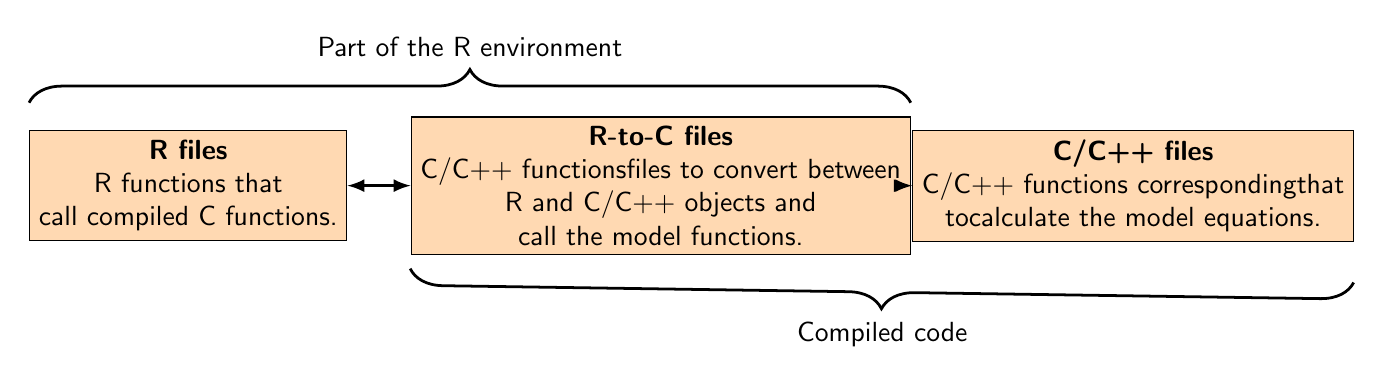
\begin{tikzpicture}[node distance=2 cm, decoration={brace}]
\tikzstyle{process} = [rectangle, minimum width=3 cm, minimum height=1 cm, text centered, draw=black, fill=orange!30]
\node (R)  [process, align=center] {\textbf{R files}\\R functions that\\call compiled C functions.};
\node (RC) [process, align=center, right of=R, xshift=4 cm] {\textbf{R-to-C files}\\C/C++ \replaced{functions}{files} to convert between\\R and C/C++ objects and\\call the model functions.};
\node (C)  [process, align=center, right of=RC, xshift=4 cm] {\textbf{C/C++ files}\\C/C++ functions \replaced{corresponding}{that}\\ \replaced{to}{calculate} the model equations.};

\draw [latex-latex, line width=1.1 pt] (R) -- (RC);
\draw [latex-latex, line width=1.1 pt] (RC) -- (C);

\draw [decoration={brace, raise=10 pt, amplitude=12 pt}, decorate, line width=1 pt] (R.north west) -- node[above=23 pt] {Part of the R environment} (R.north -| RC.east);
\draw [decoration={brace, raise=10 pt, amplitude=12 pt, mirror}, decorate, line width=1 pt] (R.south -| RC.west) -- node[below=23 pt] {Compiled code} (RC.south -| C.east);

%\draw [decoration={brace, raise=10 pt, amplitude=10 mm}, decorate, line width=1 pt] (R.north west) -- (R.north -| RC.east) {Part} (RC);
%5\draw[decoration={brace, raise=-10 pt, mirror, amplitude=10 mm, raise=5pt},decorate]
%  (RC.north -| RC.west -- node[right=6pt] {$AAAAAAAAAAAAAAAAa$} (C);
  
\end{tikzpicture}
\end{center}
\end{figure}

R code should be written so that it only checks validity of arguments and calls R-to-C functions. R-to-C code should only provide error checking and call C/C++ functions.\comment{Is \code{c4photo()} in R\_c4photo.cpp an aberration then?  It assumes several of its SEXP arguments may have length greater than one and iterates through them, calling \code{c4photoC()} for each index.} That is, R and R-to-C functions should only provide a way to access the models written in C/C++, and no modeling should be done in R or R-to-C code.

\subsection{Writing new models}
The C++ code is designed so that the functions have notation similar to the mathematical model. That is, they look like $\frac{dX_{t,cd}}{dt} = h(X_{t})$. In BioCro, functions that implement $h(X_{t})$ are called modules.

As in the R code, both $\frac{dX_{t,cd}}{dt}$ and $X_{t}$ are represented as \added{sets of} key-value pairs. The data type used for this in C++ is a \code{state\_map}. As an example, to model leaf growth rate as half of canopy assimilation rate going to leaves\comment{\emph{canopy assimilation rate going to leaves:} Would it be proper to just say ``leaf-canopy assimilation rate''?}, the following code would be used:

\begin{minipage}{\linewidth}
\begin{center}
\begin{lstlisting}[language=c++]
state_map simple_leaf_growth::do_operation(state_map const &s) const
    state_map partial_rates_of_change;
    partial_rates_of_change["Leaf"] = s.at("Assim") * 0.5;
    return partial_rates_of_change;    
}
\end{lstlisting}
\end{center}
\end{minipage}

The function is named \code{do\_operation} and is part of the \code{simple\_leaf\_growth} model.\comment{It's not clear to me if you still mean model here in the original sense from sections 1.1 and 1.2 or whether you have a more computer-software-specific meaning in mind.} It accepts a \code{state\_map} named \code{s} and returns a \code{state\_map} named \code{partial\_rates\_of\_change}. The current state of the model ($X_t$), is passed in as \code{s}. The \code{const} keywords are required, but do not need to be understood here. Canopy assimilation rate is calculated in a different part of the model, and it is stored in \code{s} with the name \code{Assim}. To access values in a \code{state\_map}, use the \code{at()} function. To assign a value to parameters within a \code{state\_map}, use the \code{[]} operator. Here, half of the assimilation rate is added to the partial rate of change of leaf growth. Note that \replaced{the call statement}{when called, the code} has the same form as $\frac{dX_{t,cd}}{dt} = h(X_{t})$:

\begin{center}
\begin{lstlisting}[language=c++]
rates_of_change = simple_leaf_growth(current_state);  
\end{lstlisting}
\end{center}
\comment{Shouldn't it be \code{rates\_of\_change = simple\_leaf\_growth::do\_operation(current\_state);}?}

A separate module can be written to describe loss of leaf mass. To describe leaf loss as a fraction of the current leaf mass, the following model could be used:

\begin{center}
\begin{lstlisting}[language=c++]
state_map fractional_leaf_loss::do_operation(state_map const &s) const
    state_map partial_rate_of_change;
    partial_rate_of_change["Leaf"] = -s.at["Leaf"] * 0.01;
    return partial_rate_of_change;    
}
\end{lstlisting}
\end{center}

The addition of the partial rates is handled elsewhere in the code, and does not need to be handled when writing new modules. This design allows one to write modules that operate independently, so that one does not need to know how the entire model works in order to modify a specific aspect of the model. To write a new module, one needs to know only what parameters are defined in the state ($X$), which is a relatively short list.

\end{document}

